\section{Teljes képernyős mód}

Az eddig elkészült alkalmazás már képes videofájlok lejátszására, illetve alapvető vezérlési funkciókat is ismer, azonban a szoftver egy fontos része hiányos, tekintve, hogy elsősorban film lejátszására ajánlott, ami a tényleges teljes képernyős mód. A jelenlegi verzió már beépítetten támogatja a teljes képernyős módot, azonban csak olyan módon, hogy a felső kezelősáv, és a tálca végig látszódik, idő elteltével sem tűnik el. Ez bármilyen médiatartalom hosszútávú nézése során rendkívül zavaró, hasznos képernyőfelületet takar el feleslegesen. Ezt úgy orvosoltam, hogy a teljes képernyő gomb megnyomásakor a videó kitölti a képernyőfelület egészét, eltüntetve ezzel a menüsávot és a kezelőpanelt. Ehhez szükség volt a következő kódsor beillesztésére az alkalmazás forráskódjába, amely a natív \textit{Win32 API}-t használja a teljes képernyős mód elérésére.

\begin{verbatim}
FullScreenStrategy fullScreenStrategy =
   new Win32FullScreenStrategy(mainFrame);
\end{verbatim}

Az új funkció alkalmazása azonban egy új problémát vetett fel: ha a képernyő egésze foglalt, és nem jelenik meg a kezelősáv, akkor a felhasználó nem tudja a teljes képernyős módot bezárni. Ennek megoldására egy általánosan használt módszert alkalmaztam. Ha a felhasználó a kurzort a képernyő alsó felére húzza, a vezérlőpanel megjelenik, és megjelenítve is marad mindaddig, amíg a felhasználó el nem távolítja az alsó területről a kurzort. Itt egyszerűen a teljes képernyős mód gombjára kattintva kiléphetünk abból. Ennek a megvalósításáért, illetve a panel megjelenítésének kezeléséért egy \textit{MouseListener} felel. Amennyiben az alkalmazás teljes képernyős módban van, a figyelő ellenőrzi a kurzor aktuális Y koordináta szerinti pozícióját, és ha ez egy bizonyos szám alatti, vagy feletti, akkor a szerint jeleníti meg, valamint rejti el a vezérlőpanelt, illetve ennek megfelelően igazítja a vásznat és a feliratokat.

\begin{verbatim}
@Override
public void mouseMoved(MouseEvent e) {
   if(mediaPlayer.isFullScreen()) {
        if (e.getYOnScreen() < 1060
        && controlsPanel.isVisible()) {
            controlsPanel.setVisible(false);
            ((SubtitleOverlay)(mediaPlayer.getOverlay()))
            .decreaseYOffset(controlsPanel.getHeight());
        } else if (e.getYOnScreen() >= 1060
        && !controlsPanel.isVisible()) {
            controlsPanel.setVisible(true);
            ((SubtitleOverlay(mediaPlayer.getOverlay()))
            .increaseYOffset(controlsPanel.getHeight());
        }
    }
}
\end{verbatim}

Ezen felül további kényelmi funkciókat is implementáltam a hatékonyabb teljes képernyős mód kezeléséért. A mód aktiválható a vászonra történő dupla kattintással, és meg is szüntethető ugyanezzel a módszerrel. Ehhez szintén egy \textit{MouseListener}-t hívtam segítségül, amely figyeli az egymás utáni kattintások számát, és ha ez az érték kettővel egyenlő kettővel, be- valamint kilép a teljes képernyős módból. Egy másik megvalósított segédfunkció az \textit{Esc} gombbal történő vezérlés. Amennyiben az alkalmazás teljes képernyőn fut, a mód megszakítható az \textit{Esc} gomb egyszeri megnyomásával. Mindkét lehetőség kényelmesebb, gyorsabb használatot tesz lehetővé, ezzel is növelve a felhasználói komfortérzetet.

\begin{figure}
  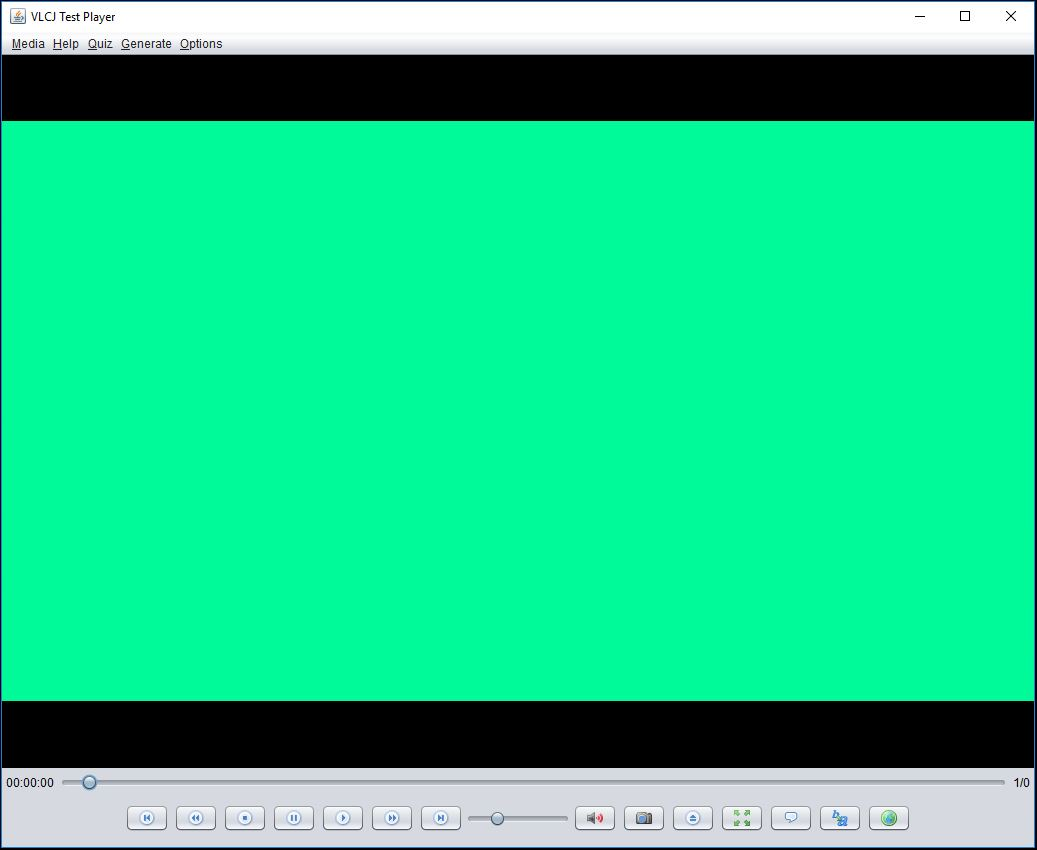
\includegraphics[width=\linewidth]{images/full_screen.jpg}
  \caption{Teljes képernyős mód a módosított FullScrennStrategy előtt}
  \label{fig:full_screen}
\end{figure}

